\documentclass[11pt]{article}
\usepackage[utf8]{inputenc}
\usepackage{amsmath,amsthm,amsfonts,amssymb,amscd}
\usepackage{multirow,booktabs}
\usepackage[table]{xcolor}
\usepackage{fullpage}
\usepackage{lastpage}
\usepackage{enumitem}
\usepackage{fancyhdr}
\usepackage{mathrsfs}
\usepackage{wrapfig}
\usepackage{setspace}
\usepackage{calc}
\usepackage{multicol}
\usepackage{cancel}
\usepackage[retainorgcmds]{IEEEtrantools}
\usepackage[margin=3cm]{geometry}
\usepackage{amsmath}
\newlength{\tabcont}
\setlength{\parindent}{0.0in}
\setlength{\parskip}{0.05in}
\usepackage{empheq}
\usepackage{framed}
\usepackage[most]{tcolorbox}
\usepackage{xcolor}
\colorlet{shadecolor}{orange!15}
\parindent 0in
\parskip 12pt
\geometry{margin=1in, headsep=0.25in}
\theoremstyle{definition}
\newtheorem{defn}{Definition}
\newtheorem{reg}{Rule}
\newtheorem{exer}{Exercise}
\newtheorem{note}{Note}

\usepackage[superscript,biblabel]{cite}
\usepackage{hyperref}
\hypersetup{colorlinks,linkcolor={blue},citecolor={blue},urlcolor={orange}} 

\usepackage{graphicx}
%Path relative to the main .tex file 
\graphicspath{ {./images/} }

\title{\textbf{Emotion recognition using physiological signals}}
\author{
  Russel Shawn Dsouza\\
  171EC143
  \and
  Sathvik S Prabhu\\
  171EC146
}
\date{}

\begin{document}
  \maketitle

  \section{Introduction}
    Emotions play a critical role in the evolution of consciousness and the operations of all mental processes. The different types of emotions have been shown to be related to various levels of consciousness\cite{izard_emotion_2009}.
    Positive emotions help improve human health and work efficiency, while negative emotions may cause health problems.
    Experiences of negative emotions are inevitable and at times useful. 
    Even so, when extreme, prolonged, or contextually inappropriate, negative emotions can trigger a wide array of problems for individuals and for society. 
    Fear and anxiety, for instance, fuel phobias and other anxiety disorders \cite{ohman_automatic_1993} and together with acute and chronic stress may compromise immune functioning and create susceptibilities to stress-related physical disorders \cite{oleary_stress_1990}. 
    For some individuals, sadness and grief may swell into unipolar depression \cite{nolen-hoeksema_response_1993}, which when severe can lead to immunosuppression \cite{oleary_stress_1990}, loss of work productivity \cite{coryell_enduring_1993}, and suicide \cite{chen_lifetime_1996}. 
    Anger and its poor management have been implicated in the etiology of heart disease\cite{barefoot_hostility_1983, fredrickson_hostility_2000, scheier_person_1995} and some cancers\cite{eysenck_cancer_1994, greer_psychological_1975}, as well as in aggression and violence, especially in boys and men\cite{buss_evolution_2016, lemerise_development_2008}.

    Emotion recognition helps to qualitatively and quantitavely understand emotions, providing tools to aid the cure of a lot of mental diseases and disorders. 

    In general, emotion recognition methods can be classified into two major categories. 
    The first is using human physical signals such as facial expression, speech, gesture, posture, etc., which has the advantage of easy collection and has been studied for years. 
    However, their reliability cannot be guaranteed, as it’s relatively easy for people to control physical signals like facial expressions or speech to hide their real emotions especially during social communications.

    The other category is using internal signals i.e. the physiological signals, which include the electroencephalogram(EEG), temperature(T), electrocardiogram(ECG), electromyogram(EMG), galvanic skin response(GSR), respiration(RSP).
    Physiological signals are generated in response to the Central Nervous System (CNS) and the Autonomic Nervous System (ANS) of human body, in which emotion changes, according to Cannon’s theory\cite{cannon_james-lange_1927}.
    One of the major benefits of the latter method is that the CNS and the ANS are largely involuntarily activated and therefore cannot be easily controlled.

  \section{Motivation}
    Emotion recognition has been applied in many areas such as safe driving\cite{de_nadai_enhancing_2016}, health care\cite{guo_pervasive_2013} especially mental health monitoring\cite{verschuere_psychopathy_2006}, social security\cite{noauthor_facial_nodate}, and so on. 
    Post Traumatic Stress Disorder (PTSD), depression and suicide are major psychiatric problems in both military and civilians\cite{bryan_combat_2013, tarrier_suicide_2004} and our system could help us better understand these problems with reliable data.
    Additionally, in rehabilitation applications, guiding patients through their rehabilitation training while adapting to the patients emotional state, is shown to be highly motivating and to lead to a faster recovery\cite{evans_positive_2011}.

    Many current methods use facial expressions to recognize the emotional states but they are not reliable as they can be deliberately falsified\cite{cannon_james-lange_1927}.
    This system can be used to monitor old aged people and those with intellectual disabilities like autism spectrum disorder(ASD). 
    These people are the primary target for an effective emotion recognition system as they find it difficult to recognize, express and control emotions\cite{sparks_brain_2002}.
    The acquisition of the physiological signals requires less energy and storage capacity and opens pathways for future low cost solutions. 
    The proposed system can also be used in human-computer interaction for machines to better understand humans\cite{molina_emotional_2009}. 
    Using the same system, various bio-signals can be bonded together to produce identification clues which can be used in domains like defence and banking\cite{kim_biometric_2009}.

  \section{Survey of State of the Art}
    There are different models followed for emotion recognition. 
    The Eckman's model is based on six discrete basic emotions: Happiness, Sadness, Surprise, Fear, Anger and Disgust\cite{ekman_universals_1987}. 
    The Plutchik's model uses eight fundamental emotions: Joy, Trust, Fear, Surprise, Sadness, Disgust, Anger and Anticipation\cite{plutchik_nature_2001}. 
    The third model\cite{russell_evidence_1977} focuses on two dimensional evaluation, like the valence-arousal model\cite{soleymani_multimodal_2012}.

    Many researchers have only analysed the performance of their algorithms on datasets and have not done a real life implementation of them.
    Cheng et al.\cite{cheng_novel_2017} have implemented a real time ecg based detection of negative emotions using the Bio Vid Emo DB dataset and they have obtained an accuracy of 79.46\%. 
    Mishra et al.\cite{mishra_real_2017} have used speech signals to detect emotions - Happy, Sad, Anger, Neutral and they reported an accuracy of 95\% using a Raspberry Pi III.
    Guo et al.\cite{guo_heart_2016}have used PCA and SVM to classify emotions into negative and positive states using Heart Rate Variability(HRV) features with an accuracy of 71.4\%.
    Now we cite the work done using the MAHNOB-HCI dataset\cite{soleymani_multimodal_2012}. 
    Ben and Lachiri\cite{ben_emotion_2017} have obtained accuracies of 67.5\% for arousal and 68.75\% for valence using have used ECG, SKT, GSR and RESP . They have implemented the classification stage using the SVM RBF kernel on a Raspberry Pi III Model B.
    Ferdinando et al.\cite{ferdinando_comparing_2016} compared ECG and HRV features and reported that dominant frequencies based on
    bivariate empirical mode decomposition (BEMD) analysis gave better accuracies than standard HRV analysis.
   
  \newpage
  \section{Features we wish to implement}
    We plan to 
    \begin{itemize}
      \item record physiological signals from subjects (ECG, GSR, SKT) and send it to the cloud for processing.
      \item classify the signals into two emotional states - Arousal (high, low) and Valence (negative, positive)\cite{ben_emotion_2017}.
      \item display the results on a monitor connected to the Raspberry Pi
      \item develop an app which shows the results and the ECG waveform of the subject.
    \end{itemize}

  \section{Implementation Details}
    We aim to have wearable sensors for our method. The physiological data is acquired from the subject using the ECG, GSR and SKT sensors and sent to a  \href{https://www.raspberrypi.org/}{Raspberry Pi}. We are using the recent \href{https://mahnob-db.eu/hci-tagging/}{ MAHNOB-HCI dataset}\cite{soleymani_multimodal_2012} for training our model. It contains the reponses and physiological data (ECG, GSR, SKT) of 30 participants after inducing their emotional states by showing them stimulating movies. 
    Studies have found this dataset to perform better than other common datasets and they attribute this to stronger emotions being induced in this dataset\cite{simon_selection_2016}.

    The model is built using \href{https://github.com/pytorch/pytorch}{PyTorch} and \href{https://github.com/pytorch/ignite}{ignite}. PyTorch is a deep learning framework by facebook and ignite is a framework that provides useful abstractions for PyTorch. The mobile app is built using \href{https://facebook.github.io/react-native/}{React Native} and \href{https://expo.io/}{Expo}, so that the app can have the same codebase for both iOS and Android. Waveform data from the sensors is sent to \href{https://aws.amazon.com/iot/}{AWS IoT} on the cloud to be processed by the model.

    \begin{figure}[h]
      \centering
      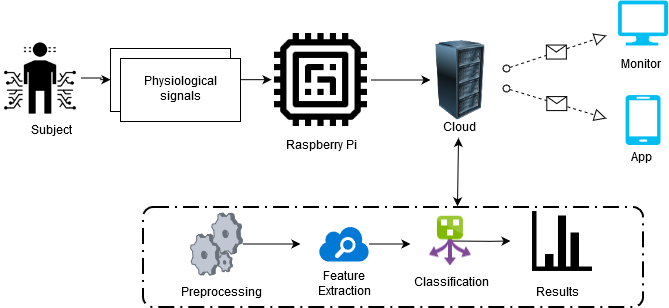
\includegraphics[scale=0.6]{schematic}
      \caption{Block diagram of proposed implementation}
    \end{figure}
    
  \newpage
  \section{Project Timeline}
    \begin{figure}[h]
      \centering
      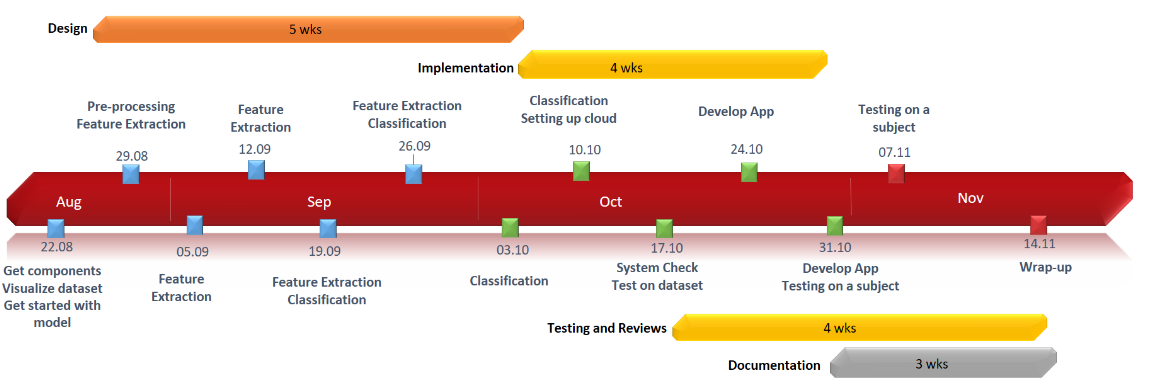
\includegraphics[width=\textwidth, scale=1.5]{pert_chart}
      \caption{PERT Chart}
    \end{figure}
  
  \bibliography{bibliography}
  \bibliographystyle{ieeetr}

\end{document}
